%
% File acl2020.tex
%
%% Based on the style files for ACL 2020, which were
%% Based on the style files for ACL 2018, NAACL 2018/19, which were
%% Based on the style files for ACL-2015, with some improvements
%%  taken from the NAACL-2016 style
%% Based on the style files for ACL-2014, which were, in turn,
%% based on ACL-2013, ACL-2012, ACL-2011, ACL-2010, ACL-IJCNLP-2009,
%% EACL-2009, IJCNLP-2008...
%% Based on the style files for EACL 2006 by 
%%e.agirre@ehu.es or Sergi.Balari@uab.es
%% and that of ACL 08 by Joakim Nivre and Noah Smith

\documentclass[11pt,a4paper]{article}
\usepackage[hyperref]{acl2020}
\usepackage{times}
\usepackage{latexsym}
\renewcommand{\UrlFont}{\ttfamily\small}

\usepackage{array, booktabs}
\usepackage{geometry}
\usepackage{multirow}

% This is not strictly necessary, and may be commented out,
% but it will improve the layout of the manuscript,
% and will typically save some space.
\usepackage{microtype}

\aclfinalcopy % Uncomment this line for the final submission
%\def\aclpaperid{***} %  Enter the acl Paper ID here

%\setlength\titlebox{5cm}
% You can expand the titlebox if you need extra space
% to show all the authors. Please do not make the titlebox
% smaller than 5cm (the original size); we will check this
% in the camera-ready version and ask you to change it back.

\newcommand\BibTeX{B\textsc{ib}\TeX}

\title{Experiment Protocol for CS224U, Spring 2020.}

\author{Abhishek Goswami \\
  Microsoft / Redmond, WA \\
  \texttt{agoswami@microsoft.com}}

%\author{First Author \\
  %Affiliation / Address line 1 \\
  %Affiliation / Address line 2 \\
  %Affiliation / Address line 3 \\
  %\texttt{email@domain} \\\And
  %Second Author \\
  %Affiliation / Address line 1 \\
  %Affiliation / Address line 2 \\
  %Affiliation / Address line 3 \\
  %\texttt{email@domain} \\}

\date{}

\begin{document}

\maketitle

\begin{abstract}

This document sets the experiment protocol for CS224U, Spring 2020 quarter. 

\end{abstract}


%\section{General Problem}
\label{sec:general problem}

The general problem we are trying to address is Natural Language Inference (NLI), the task of determining if a premise sentence entails a hypothesis statement. In recent years, Transformer-based models have been shown to be very effective in this task.

In particular, we study the problem of Adversarial NLI \cite{nie2019adversarial} which poses a challenge to the state-of-the-art models. We then study the structural properties of a popular deep learning model, BERT \cite{devlin-etal-2019-bert} from the perspective of what it does \cite{michel2019sixteen, rogers2020primer, clark2019does}.
 
%\section{Article Summary}
\label{sec:articlesummary}

In this section we provide summaries of several papers.

\subsection{\cite{devlin-etal-2019-bert}}
\label{subsec:devlin-etal}

\subsection{\cite{nie2019adversarial}}
\label{subsec:nie2019adversarial}

\subsection{\cite{michel2019sixteen}}
\label{subsec:michel2019sixteen}

\subsection{\cite{rogers2020primer}}
\label{subsec:rogers2020primer}

\subsection{\cite{clark2019does}}
\label{subsec:clark2019does}

\subsection{\cite{vaswani2017attention}}
\label{subsec:vaswani2017attention}

\subsection{\cite{mccoy2019right}}
\label{subsec:mccoy2019right}

%\section{Compare And Contrast}
\label{sec:compareandcontrast}

Point out the similarities and differences of the papers. Do they agree with each other? Are results seemingly in conflict? If the papers address different subtasks, how are they related? (If they are not related, then you may have made poor choices for a lit review...). This section is probably the most valuable for the final project, as it can become the basis for a lit review section..

%\section{Future Work}
\label{sec:futurework}

We identify some strands of work for future:

\begin{enumerate}

\item
We want to build Transformer based models for Adverserial NLI and compare them with non-deep learning models. We hope that a comparison of these approaches for the task of Adverserial NLI will give us some grounds to build up more intuition about the Adversarial NLI task.
 
\item
We want to explore whether the role attributed to multi-headed attention in the non-adversarial setting also holds true for adversarial models. The hunch we have is that attention heads will have a markedly different role in the adversarial setting given the nature of the data.

\item
We want to study the role of positional embeddings in the adversarial setting. 

\end{enumerate}

The author is a SCPD student in a single person team. There are no external collaborators. We are looking forward to a mentor being assigned to us. We are are not sharing this project with any other class.

\section{Hypothesis}
\label{sec:hypothesis}

%A statement of the project's core hypothesis or hypotheses.

Natural language inference (NLI) is the task of determining if a natural language hypothesis can be inferred from a given premise in a justifiable manner. Existing models perform well at standard evaluations for NLI, achieving impressive results in leaderboards such as GLUE. However, a growing body of evidence \cite{mccoy2019right, glockner2018breaking} shows that state-of-the-art models learn to exploit spurious statistical patterns in datasets instead of learning meaning in the flexible and generalizable way. NLI adversarial evaluations, where existing state-of-the art NLI systems are evaluated on a completely unseen new test dataset, further exposes these concerns. State-of-the art NLI systems perform quite poorly in the adversarial evaluation setting \cite{nie2019adversarial}, reflecting that such systems do not represent true competence at natural language understanding. This begs the question: If a system fails an NLI adversarial evaluation, is it a failing of the model or of the dataset used to develop the model?

In this work, we hypothesize that the failings in the adversarial evaluation setting come from the dataset used to develop the model. Standard evaluations in NLI typically use datasets generated using a single generation process. We argue that these standalone, per-dataset generation processes encode latent signals in the premise/hypothesis construction. This leads to favorable results in the standard evaluation setting, but fail spectacularly in the the adversarial evaluation setting. We believe this can be improved by using a mix of multiple weakly-supervised datasets during the training process. This setting enables us to leverage several related sentence pair datasets, while avoiding per-dataset statistical concerns.


  





\section{Data}
\label{sec:data}

A description of the dataset(s) that the project will use for evaluation.
\section{Metrics}
\label{sec:metrics}

A description of the metrics that will form the basis for evaluation. We require at least one of these to be quantitative metrics, but we are very open-minded about which ones you choose. In requiring this, we are not saying that all work in NLU needs to be evaluated quantitatively, but rather just that we think it is a healthy requirement for our course.
\section{Models}
\label{sec:models}

A description of the models that you'll be using as baselines, and a preliminary description of the model or models that will be the focus of your investigation. At this early stage, some aspects of these models might not yet be worked out, so preliminary descriptions are fine.
\section{General Reasoning}
\label{sec:reasoning}

%An explanation of how the data and models come together to inform your core hypothesis or hypotheses.

\begin{figure*}
	\centering
		\subfloat[{\small BERT}]{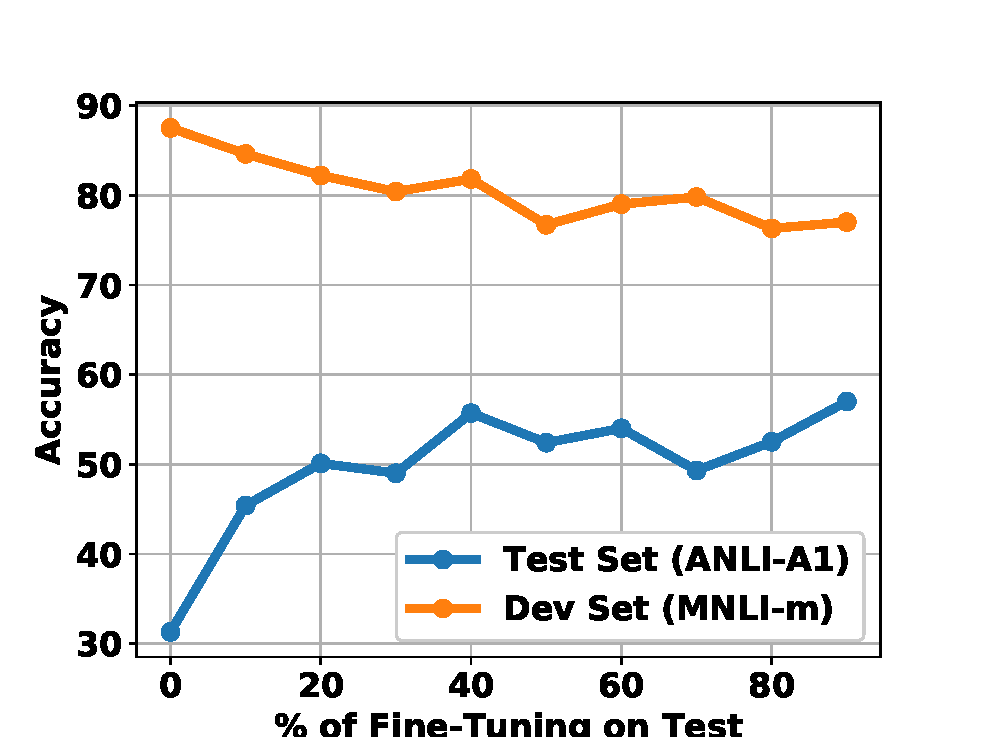
\includegraphics[width=0.45\textwidth]{Figs4Paper/percentage_finetuned_vs_accuracy_roberta.eps}}
		\subfloat[{\small RoBERTa}]{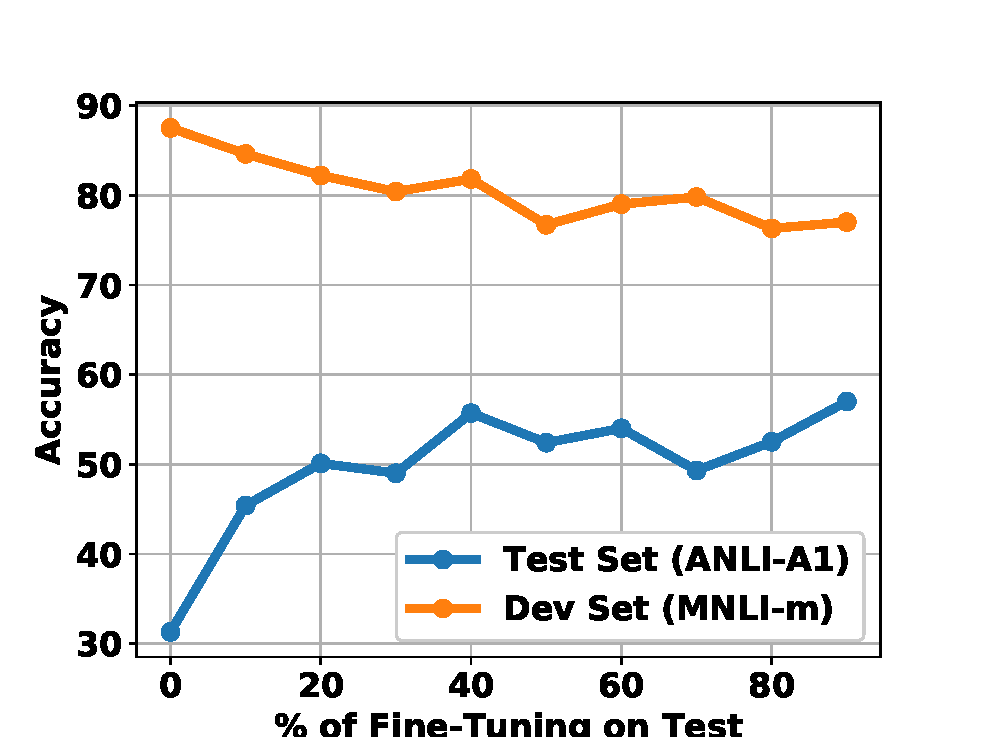
\includegraphics[width=0.45\textwidth]{Figs4Paper/percentage_finetuned_vs_accuracy_roberta.eps}}
	\caption{Inoculation by fine-tuning on the test set}
	\label{fig:inoculation}
\end{figure*}

Our hypothesis is that that the failings in NLI adversarial evaluation come from the use of singular datasets used to develop the model. To avoid this we introduce a wide range of datasets as part of our train set.  On the model side, we have two state-of-the art models: BERT\textsubscript{BASE} and RoBERTa\textsubscript{BASE} which perform exceedingly well in standard NLI tasks. By diversifying our training data, we aim to show that these two models can also do well in the NLI adversarial evaluation setting.
\section{Progress Summary}
\label{sec:progress}

% what you have been done \ref{table:accuracy}, what you still need to do, and any obstacles or concerns that might prevent your project from coming to fruition 



In this section, we report the progress we have made so far. Table \ref{table:accuracy} shows a comprehensive view of the experiments done so far.

\subsection{Training on MNLI only}
\label{subsec:trainmnli}

A random guessing strategy gives a accuracy of 33.3\% on both the Dev and Test sets which is intuitive given that we have 3 labels which are uniformly distributed (See Section \ref{sec:data}). 

Compared to Random, our Baseline model does better on the Dev set indicating it has picked up signal from the MNLI training data. However, it does worse than Random in the adversarial evaluation setting when evaluated on the ANLI-A1 test set. We see similar behaviour for both the `simple' Transformer-based models, . When trained on MNLI data both BERT\textsubscript{BASE} and RoBERTa\textsubscript{BASE} do remarkably well on the Dev set, but do quite poorly on the ANLI-A1 test set. In this setting, only RoBERTa\textsubscript{LARGE} is able to outperform Random on the Test set.

\subsection{Analyzing Transformer models on Adversarial data}
\label{subsec:analyzetransformeradversarial}

We try to understand what Transformed-based models are doing from two perspectives (a) Error analysis and (b) Role of the attention heads. For this we continue to use models trained on MNLI only. \\

\noindent {\bf Error Analysis:} We look at some examples where \textit{both} BERT\textsubscript{BASE} and RoBERTa\textsubscript{BASE} are wrong, while being in perfect agreement with each other. Table \ref{table:erroranalysis} shows one example from each such category. This leads to a few observations:

\begin{itemize}
	\item Adversaries are exploiting numerical abilities, including in some cases the inability of the models to do math.  
	\item Both models seem to biased towards predicting the \texttt{contradiction} label, with the number of predicted \texttt{contradiction} labels being almost 20\% more than the number of \texttt{entailment} labels.
	
\end{itemize}

\noindent {\bf Attention heads:} We look at the role of attention heads for both the standard evaluation setting (using MNLI-m as the target dataset) and for the adversarial evaluation setting (using ANLI-A1 as the target dataset). In \cite{michel2019sixteen} the authors note that at test time, many attention heads can be re-
moved individually without impacting model performance. In Section \ref{subsec:trainmnli} we noted that a BERT\textsubscript{BASE} trained on MNLI data did did worse than Random on the ANLI-A1 test set. Interestingly, we saw that we had to prune almost 90\% of the attention heads of the model for it to match Random. Figure \ref{fig:attentionheads} accuracy of a BERT\textsubscript{BASE} model as a function of the number of attention heads. The BERT\textsubscript{BASE} model was trained on MNLI only data.

\subsection{Training on multiple data sources}
\label{subsec:trainmultiple}

In line with our stated hypothesis, we now mix multiple datasets to construct our train data. The hope is that this will enable us to capture a diverse range of latent signals from multiple data generation processes. For efficiency purposes, we currently sample from the data ratio to gain an intuition on how well our models are doing. In this setting, we only report the results for the BERT\textsubscript{BASE} and RoBERTa\textsubscript{BASE} models

Unfortunately, so far our results are in line with the observations in Section \ref{subsec:trainmnli}. Both the transformer models are doing remarkably well on the Dev set, but poorly on the ANLI-A1 Test set.

\subsection{Advice}
\label{subsec:advice}

Any suggestions on how to further improve the models would be highly welcome. Specifically in adressing the limitation of models with respect to their numerical abilities as noted above in Section \ref{subsec:analyzetransformeradversarial}


\bibliography{acl2020}
\bibliographystyle{acl_natbib}

\end{document}
